\documentclass[a3paper]{article}
\usepackage[left=2mm,top=1cm,right=0mm,bottom=0mm]{geometry}
% \documentclass[border=0]{standalone}
\usepackage{tikz}
\usepackage{xcolor}
\definecolor{pGreen}{HTML}{006633}
\definecolor{sgbGreen1}{HTML}{66cc99}
\definecolor{sgbGreen2}{HTML}{ccffcc}

\definecolor{pRed}{HTML}{cc0033}
\definecolor{sgbRed}{HTML}{cc6688}
\definecolor{sgbRed2}{HTML}{FF99CC}

\definecolor{sgbGrey}{HTML}{333333}
\definecolor{sgbGrey2}{HTML}{996666}
\definecolor{sgbGrey3}{HTML}{999966}

\begin{document}
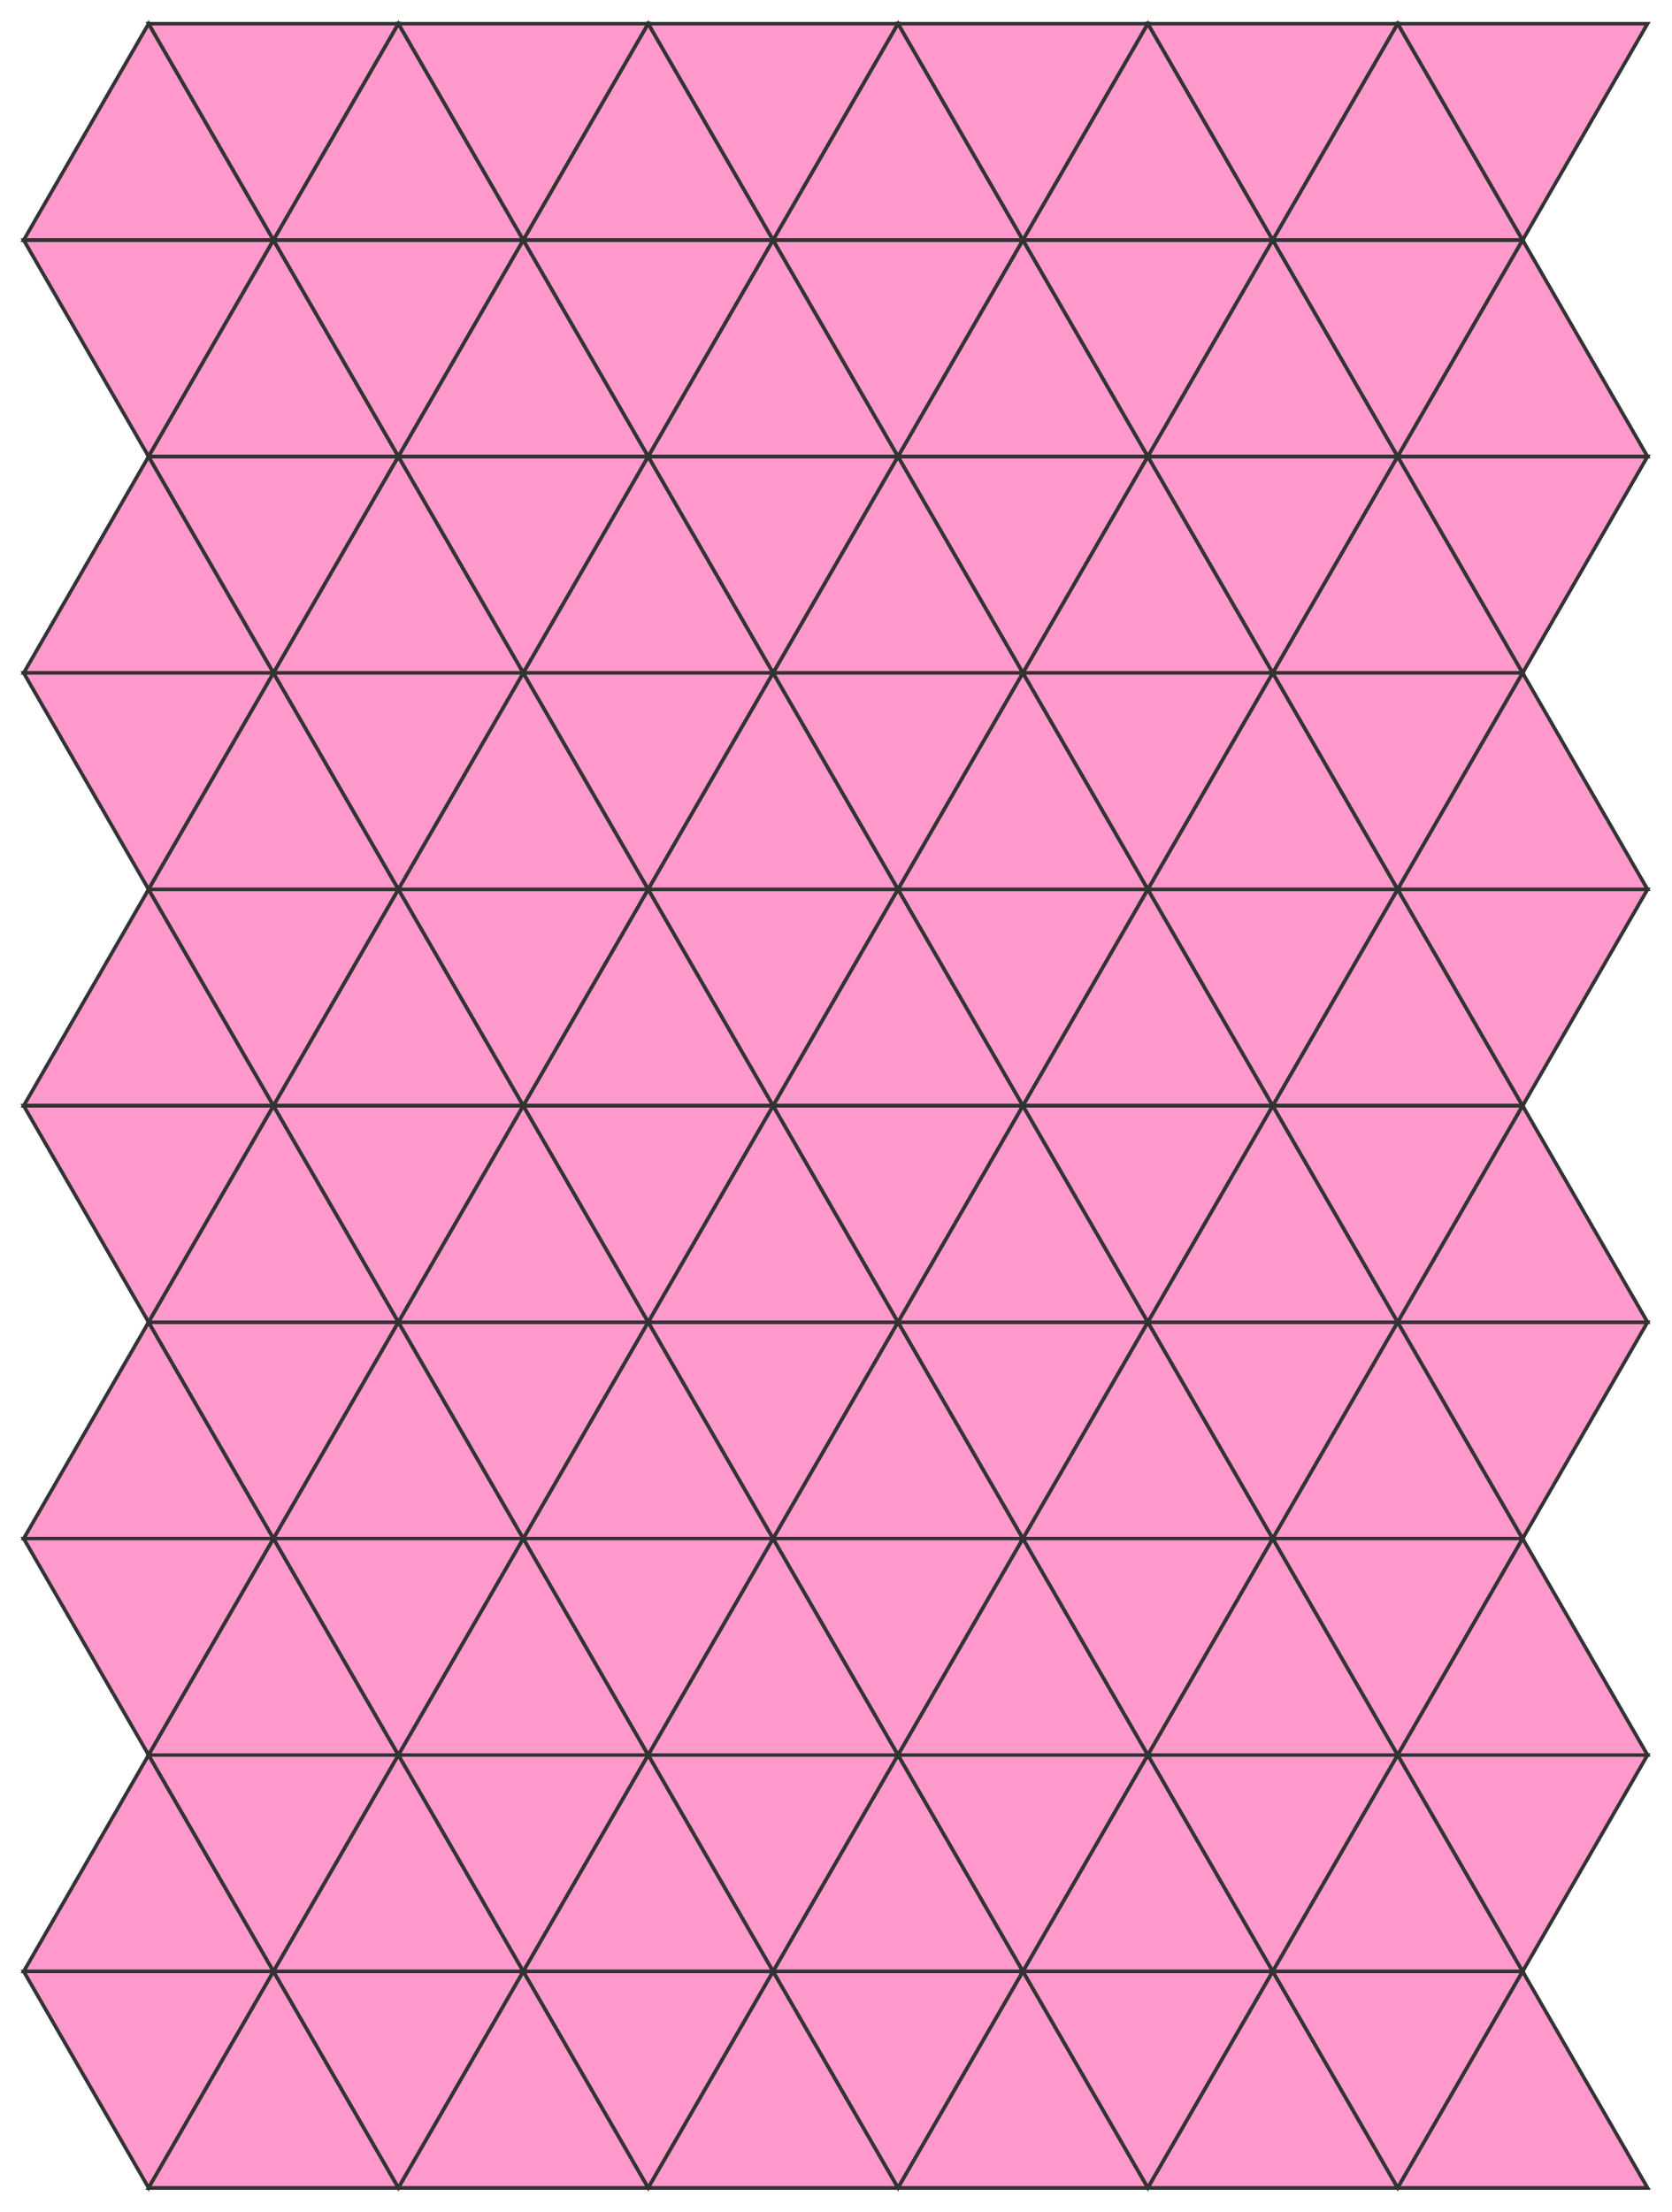
\begin{tikzpicture}
    \pgfmathsetmacro{\w}{4}
    \tikzset{
        triangle/.pic={
            \filldraw[sgbRed2,draw=sgbGrey,ultra thick] (0,0) --++(0:\w)--++(120:\w)--cycle;
            \filldraw[sgbRed2,draw=sgbGrey,ultra thick] (\w,0) --++(60:\w)--++(180:\w)--cycle;
            \filldraw[sgbRed2,draw=sgbGrey,ultra thick] ({\w*cos(60)},{-\w*sin(60)}) --++(60:\w)--++(180:\w)--cycle;
            \filldraw[sgbRed2,draw=sgbGrey,ultra thick] ({\w*cos(60)},{-\w*sin(60)}) --++(0:\w)--++(120:\w)--cycle;
        }
    };
    \foreach \col in {0,...,5}{
        \foreach \row in {0,...,4}{
        \draw(\col*\w,{2*\row*\w*sin(60)}) pic {triangle};}
        }
\end{tikzpicture}
\end{document}

\foreach \row in {0,...,3}{
    \draw (0,{\row*sqrt(3)/2}) --++ (0:3);
    \draw (\row,0) --++ (60:4);
    \draw (\row,0) --++ (120:4);}